\documentclass[11pt]{article}

% Language setting
\usepackage[turkish]{babel}
\usepackage{pythonhighlight}

\usepackage[a4paper,top=2cm,bottom=2cm,left=2cm,right=2cm,marginparwidth=2cm]{geometry}

% Useful packages
\usepackage{amsmath}
\usepackage{graphicx}
\usepackage[colorlinks=true, allcolors=blue]{hyperref}
\usepackage{verbatim}
\usepackage{fancyhdr} % for header and footer
\usepackage{titlesec}
\usepackage{parskip}

\setlength{\parindent}{0pt}

\titleformat{\subsection}[runin]{\bfseries}{\thesubsection}{1em}{}

\pagestyle{fancy} % activate the custom header/footer

% define the header/footer contents
\lhead{\small{23BLM-4014 Yapay Sinir Ağları Ara Sınav Soru ve Cevap Kağıdı}}
\rhead{\small{Dr. Ulya Bayram}}
\lfoot{}
\rfoot{}

% remove header/footer on first page
\fancypagestyle{firstpage}{
  \lhead{}
  \rhead{}
  \lfoot{}
  \rfoot{\thepage}
}
 

\title{Çanakkale Onsekiz Mart Üniversitesi, Mühendislik Fakültesi, Bilgisayar Mühendisliği Akademik Dönem 2022-2023\\
Ders: BLM-4014 Yapay Sinir Ağları/Bahar Dönemi\\ 
ARA SINAV SORU VE CEVAP KAĞIDI\\
Dersi Veren Öğretim Elemanı: Dr. Öğretim Üyesi Ulya Bayram}
\author{%
\begin{minipage}{\textwidth}
\raggedright
Öğrenci Adı Soyadı: Onur ÖNER\\ % Adınızı soyadınızı ve öğrenci numaranızı noktaların yerine yazın
Öğrenci No: 190401095
\end{minipage}%
}

\date{14 Nisan 2023}

\begin{document}
\maketitle

\vspace{-.5in}
\section*{Açıklamalar:}
\begin{itemize}
    \item Vizeyi çözüp, üzerinde aynı sorular, sizin cevaplar ve sonuçlar olan versiyonunu bu formatta PDF olarak, Teams üzerinden açtığım assignment kısmına yüklemeniz gerekiyor. Bu bahsi geçen PDF'i oluşturmak için LaTeX kullandıysanız, tex dosyasının da yer aldığı Github linkini de ödevin en başına (aşağı url olarak) eklerseniz bonus 5 Puan! (Tavsiye: Overleaf)
    \item Çözümlerde ya da çözümlerin kontrolünü yapmada internetten faydalanmak, ChatGPT gibi servisleri kullanmak serbest. Fakat, herkesin çözümü kendi emeğinden oluşmak zorunda. Çözümlerinizi, cevaplarınızı aşağıda belirttiğim tarih ve saate kadar kimseyle paylaşmayınız. 
    \item Kopyayı önlemek için Github repository'lerinizin hiçbirini \textbf{14 Nisan 2023, saat 15:00'a kadar halka açık (public) yapmayınız!} (Assignment son yükleme saati 13:00 ama internet bağlantısı sorunları olabilir diye en fazla ekstra 2 saat daha vaktiniz var. \textbf{Fakat 13:00 - 15:00 arası yüklemelerden -5 puan!}
    \item Ek puan almak için sağlayacağınız tüm Github repository'lerini \textbf{en geç 15 Nisan 2023 15:00'da halka açık (public) yapmış olun linklerden puan alabilmek için!}
    \item \textbf{14 Nisan 2023, saat 15:00'dan sonra gönderilen vizeler değerlendirilmeye alınmayacak, vize notu olarak 0 (sıfır) verilecektir!} Son anda internet bağlantısı gibi sebeplerden sıfır almayı önlemek için assignment kısmından ara ara çözümlerinizi yükleyebilirsiniz yedekleme için. Verilen son tarih/saatte (14 Nisan 2023, saat 15:00) sistemdeki en son yüklü PDF geçerli olacak.
    \item Çözümlerin ve kodların size ait ve özgün olup olmadığını kontrol eden bir algoritma kullanılacaktır. Kopya çektiği belirlenen vizeler otomatikman 0 (sıfır) alacaktır. Bu nedenle çözümlerinizi ve kodlarınızı yukarıda sağladığım gün ve saatlere kadar kimseyle paylaşmayınız.
    \item Bu vizeden alınabilecek en yüksek not 100'dür. Toplam aldığınız puan 100'ü geçerse, aldığınız not 100'e sabitlenecektir.
    \item LaTeX kullanarak PDF oluşturanlar öz geçmişlerine LaTeX bildiklerini de eklemeyi unutmasınlar :)
    \item Bu vizedeki soruların çözümleri ve tex dosyası için istediğiniz kadar sayıda Github repository'si oluşturabilirsiniz. Sadece yukarıda belirttiğim tarihlerde (14 Nisan 2023 saat 15:00 ile 15 Nisan 2023 saat 15:00 arasında) public yapmayı/halka açmayı ve Github profilinizi de öz geçmişinize eklemeyi unutmayın :)
    \item Bilgisayarınıza hiçbir program kurmadan, Overleaf, Google Colab, Kaggle gibi ortamlar üzerinden bu vizeyi tamamlamanız mümkün. İyi çalışmalar!!
\end{itemize}

(Ekstra 5 puan) \url{OdevinTexDosyasınınGithubLinkiniburayakoyun.com}

\newpage
\section{(Toplam 10 Puan) Hopfield Networks:}

\subsection{(2 Puan)} \textbf{ChatGPT’ye size Hopfield Network’ler ile ilgili detaylı bilgi vermesini isteyin. Sorduğunuz soruyu, ChatGPT'nin çıkartığı cevabı aşağı koyun. Bu cevapta anlamadığınız terimleri de ChatGPT’ye sorup, sorduğunuz soruları ve ChatGPT’nin verdiği cevapları da sırayla aşağı koyun.}

Soru: Hopfield Network’ler ile ilgili detaylı bilgi verir misin?\\

ChatGPT: Hopfield ağları, sinir ağları olarak bilinen yapay zeka modellerinin bir türüdür. İlk olarak John Hopfield tarafından tanıtılmıştır ve özellikle bellek ve optimizasyon sorunlarının çözümünde kullanılırlar. Hopfield ağları, birbirine bağlı bir dizi sinir hücresinden oluşur ve bu sinir hücreleri (nöronlar), giriş sinyallerini aldıklarında belirli bir şekilde etkileşime girerek bir çıktı üretirler.

Hopfield ağları, öğrenme ve hatırlama işlevleri için kullanılırlar. Bir Hopfield ağı, öğrenme sürecinde, öğrenmek istediğimiz bilgiyi (örneğin, bir dizi sayısal değer veya bir dizi kalıp) temsil eden bir dizi giriş verisi ile eğitilir. Ağ, öğrenme süreci sırasında bu giriş verisini belleğinde tutar ve daha sonra hatırlama sürecinde, ağa benzer bir giriş verisi verildiğinde, öğrenilen bilgiyi hatırlayabilir.

Hopfield ağları, aynı zamanda optimizasyon sorunlarını çözmek için de kullanılabilir. Bu durumda, ağın sinir hücreleri, optimizasyon problemine karşılık gelen bir enerji fonksiyonunu temsil ederler. Bu enerji fonksiyonu, ağın çıktılarına dayalı olarak hesaplanır ve en düşük enerji durumunu elde etmek için ağ, iteratif bir işlemle güncellenir.

Hopfield ağları, basit yapısı ve öğrenme yetenekleri nedeniyle popüler bir yapay zeka modelidir. Bununla birlikte, büyük veri kümeleri üzerinde çalışırken performans sorunları ortaya çıkabilir ve ağın hafıza kapasitesi sınırlıdır.\\

Soru: Yukarıda bahsettiğin enerji fonksiyonu ne anlama geliyor?\\

ChatGPT: Hopfield ağlarında enerji fonksiyonu, ağın sinir hücrelerinin (nöronların) çıktılarına bağlı olarak hesaplanan bir matematiksel fonksiyondur. Enerji fonksiyonu, ağın bulunduğu bir durumun enerjisini temsil eder ve bu enerji, ağın bulunduğu durumun ne kadar "iyi" olduğunu belirtir.

Enerji fonksiyonu, genellikle aşağıdaki şekilde ifade edilir:

\begin{figure}[ht!]
    \centering
    
\includegraphics[width=0.9\textwidth]{lagrida_latex_editor.png}
    \label{fig:my_pic}
\end{figure}

Burada, E enerji fonksiyonu, wᵢⱼ sinir hücreleri arasındaki bağlantıların (ağırlıkların) güçlerini ifade eden bir matrisdir. sᵢ, sinir hücresi i'nin çıkışıdır ve θᵢ ise sinir hücresi i'nin eşiği (threshold) olarak adlandırılır.

Enerji fonksiyonu, Hopfield ağlarındaki optimizasyon problemlerini çözmek için kullanılır. Ağın hedefi, enerji fonksiyonunun en düşük değerine sahip olan bir çıkış durumu bulmaktır. Bu, ağın en optimum çözümü bulduğu anlamına gelir. Enerji fonksiyonu, ayrıca ağın hatırlama işlevinde de kullanılır, çünkü öğrenilen bilgi (örneğin, bir dizi sayısal değer veya bir dizi kalıp) ağın enerji fonksiyonunda bir minimuma karşılık gelir.

\subsection{(8 Puan)} \textbf{ChatGPT’nin açıklamalarından ne anladığınızı buraya kendi kelimelerinizle özetleyin. Örneğin ``Hopfield Network nedir? Ne işe yarar? Neden bilmemiz gerekir bunu? Gerçek hayatta kullanılıyor mu?'' gibi. Anlamadığınız kısımlar varsa ve ChatGPT’nin açıklamaları yeterli gelmezse internet dahil farklı kaynaklardan araştırıp, bilgilerin doğruluğunu sorgulamakta serbestsiniz. Konuyu doğru anlayıp anlamamanız puana etki edecektir. Kullandığınız kaynakları da belirtin!}

Hopfield ağları, birbirine bağlı nöronlardan oluşan bir yapıya sahiptir. Bu ağın nöronlarından her biri bir matematiksel işlem yaparak çıktı üretmektedir. Hopfield ağları iki aşamadan oluşan bir çalışma yapısına sahip. İlk aşamada öğrendiği bilgileri depolamaktadır. Daha sonrasında ise depoladığı bilgileri geri çağırarak mevcut girdilerde kullanmaktadır. 
Hopfield ağları her ne kadar optimizasyon sorunlarını çözmek için kullanılsa da örüntü tanıma da kullanımı söz konusudur. (Kaynak: Necmettin Sezgin, "Örüntü Tanımlamada Hopfield Ağının Kullanilmasi", Journal of Life Sciences, cilt Volume 1, no. Number 2, 2012)

\section{(Toplam 10 Puan) Boltzman Machine:}

\subsection{(2 Puan)} \textbf{ChatGPT’ye size Boltzman Machine ilgili detaylı bilgi vermesini isteyin. Sorduğunuz soruyu, ChatGPT'nin çıkartığı cevabı aşağı koyun. Bu cevapta anlamadığınız terimleri de ChatGPT’ye sorup, sorduğunuz soruları ve ChatGPT’nin verdiği cevapları da sırayla aşağı koyun.}

Soru: Boltzman Machine ile ilgili detaylı bilgi ver.\\

ChatGPT: Boltzmann Machine, yapay sinir ağları alanında yaygın olarak kullanılan bir tür olup, bir tür olasılık modelidir. İsmi, fizikçi Ludwig Boltzmann'dan gelmektedir.

Bir Boltzmann Makinesi, giriş ve çıkış katmanları arasında birden çok gizli katmanı olan bir yapay sinir ağıdır. Bu katmanlar arasında, her biri diğer katmanlardaki her bir nöronla bağlantılı olan çok sayıda nöron vardır.

Bir Boltzmann Makinesi, veri örneklerini içeren bir veri kümesi üzerinde eğitilir. Makine, verilerin özelliklerini öğrenmek için girdi verileri arasındaki olasılık dağılımlarını modellemeye çalışır. Bu amaçla, makine, eğitim verilerinin bir alt kümesine dayalı olarak olasılık dağılımını hesaplar.

Bir Boltzmann Makinesi, öğrenme için sadece öğretici veri setlerine ihtiyaç duyar. Bu nedenle, öğrenmenin gerçekleştiği aşama, denetimli öğrenme yöntemlerindeki gibi doğru veya yanlış bir yanıt almakla ilgili değildir. Bunun yerine, makine, öğrenmenin gerçekleştiği aşamada, veri kümesindeki kalıpları tespit ederek ve olasılık dağılımını modelleyerek, öğrenir.

Bir Boltzmann Makinesi, diğer yapay sinir ağlarına göre daha esnek bir modele sahiptir. Çünkü, her bir nöronun hem girdi hem de çıktı bağlantıları vardır. Bu, nöronlar arasındaki etkileşimlerin çoklu yönlerde gerçekleşebileceği anlamına gelir. Bu nedenle, Boltzmann Makineleri, daha karmaşık veri kümelerindeki kalıpları tespit etmek için daha iyi bir seçenek olabilir.

Sonuç olarak, Boltzmann Makineleri, öğrenme sürecindeki veri kümesindeki kalıpları tespit eden ve olasılık dağılımını modelleyen yapay sinir ağlarıdır. Bu esnek yapısı sayesinde, daha karmaşık veri kümelerindeki kalıpları tespit etmek için daha iyi bir seçenek olabilir.\\

Soru: Peki Boltzman Makineleri kümeleme işlemlerinde mi daha iyi sonuç verir yoksa sınıflandırma işlemlerinde mi?\\

ChatGPT: Boltzmann Makineleri, hem kümeleme hem de sınıflandırma işlemlerinde kullanılabilir. Ancak, Boltzmann Makinelerinin doğru bir şekilde öğrenilmesi ve eğitilmesi, işlem yapılacak veri kümesinin özelliklerine bağlıdır.

Örneğin, veri kümesi doğal bir gruplama veya kümeleme özelliğine sahipse, Boltzmann Makineleri kümeleme işlemlerinde daha iyi sonuçlar verebilir. Bunun nedeni, Boltzmann Makinelerinin öğrenme sürecinde veriler arasındaki benzerlikleri ve farklılıkları hesaba katmasıdır. Bu özellik sayesinde, veri kümesindeki doğal gruplamaları tespit etmek ve belirlemek için kullanılabilirler.

Öte yandan, veri kümesi belirli bir sınıflandırma görevi gerektiriyorsa, Boltzmann Makineleri sınıflandırma işlemlerinde de kullanılabilir. Ancak, sınıflandırma işlemlerinde daha sık kullanılan ve başarılı sonuçlar veren yöntemler mevcuttur, örneğin, derin öğrenme modelleri ve destek vektör makineleri.

Sonuç olarak, Boltzmann Makineleri hem kümeleme hem de sınıflandırma işlemlerinde kullanılabilirler, ancak hangi yöntemin daha iyi sonuç vereceği, işlem yapılacak veri kümesinin özelliklerine bağlıdır.\\

Soru: Boltzman makinelerinin kullanıldığı örnek bir senaryo söyler misin?

ChatGPT: Boltzmann Makineleri, geniş bir yelpazede uygulamalarda kullanılabilir. Bunlar arasında, görüntü işleme, doğal dil işleme, öneri sistemleri, robotik ve finansal modelleme gibi alanlar yer alır.

Örneğin, bir öneri sistemi uygulaması düşünelim. Bu uygulama, kullanıcılara farklı filmler, kitaplar veya ürünler hakkında öneriler sunmak için kullanılabilir. Boltzmann Makineleri, kullanıcının geçmiş alımları ve tercihlerine dayanarak, kullanıcının ilgi alanlarına uygun öneriler yapmak için kullanılabilir.

Bu uygulamada, Boltzmann Makinesi, kullanıcının geçmiş tercihlerine dayalı olarak, olası filmlerin veya kitapların listesini bir olasılık dağılımı olarak modelleyebilir. Sonra, bu dağılımı kullanarak, kullanıcının ilgi alanlarına en uygun önerileri yapabilir.

Öneri sistemi uygulaması sadece bir örnek olmakla birlikte, Boltzmann Makineleri, birçok uygulama için kullanılabilir. Bu nedenle, Boltzmann Makineleri, yapay zeka ve makine öğrenmesi alanındaki önemli araçlardan biridir.

\subsection{(8 Puan)} \textbf{ChatGPT’nin açıklamalarından ne anladığınızı buraya kendi kelimelerinizle özetleyin. Örneğin ``Boltzman Machine nedir? Ne işe yarar? Neden bilmemiz gerekir bunu? Gerçek hayatta kullanılıyor mu?'' gibi. Anlamadığınız kısımlar varsa ve ChatGPT’nin açıklamaları yeterli gelmezse internet dahil farklı kaynaklardan araştırıp, bilgilerin doğruluğunu sorgulamakta serbestsiniz. Konuyu doğru anlayıp anlamamanız puana etki edecektir. Kullandığınız kaynakları da belirtin!}

Boltzman makineleri, içerisinde birçok nöronun bulunduğu birden fazla hidden layer'dan oluşmaktadır. Bir Boltzman makinesi, olasılıksal dağılımları ve gruplanmaları belirlemektedir. Bir veriye sabit bir kategori atamak yerine, o verinin hangi diğer verilere benzediğini bulmak diyebiliriz buna. 

Boltzman makineleri, iş sektöründe önemli yerlerde kullanılabilir. Öneri sistemlerinde kullanılması, birçok şirketin müşterileri doğru bir şekilde tespit edip o müşteriye yönelik özelleştirilmiş bir deneyim katmasında önemli rol oynayabilir.

\section{(Toplam 10 Puan) Markov Assumption ve Markov Chain:}

\subsection{(2 Puan)} \textbf{ChatGPT’ye size Markov assumption ve Markov Chain ilgili detaylı bilgi vermesini isteyin. Sorduğunuz soruyu, ChatGPT'nin çıkartığı cevabı aşağı koyun. Bu cevapta anlamadığınız terimleri de ChatGPT’ye sorup, sorduğunuz soruları ve ChatGPT’nin verdiği cevapları da sırayla aşağı koyun.}

Soru: Markov assumption ve Markov Chain ile ilgili detaylı bilgi ver.

ChatGPT: Markov assumption, bir olayın gelecekteki oluşumunun, yalnızca şimdiki zamandaki duruma bağlı olduğunu varsayar. Yani, geçmiş olaylar ve durumlar, gelecekteki olayların oluşumu üzerinde etkili değildir. Bu nedenle, Markov assumption, gelecekteki olayların tahmin edilmesi için bir matematiksel model oluştururken sıkça kullanılır.

Markov Chain, belirli bir durumdan başlayarak, belirli bir olasılık dağılımı ile gelecekteki durumların sırasını modelleyen bir stokastik süreçtir. Markov Chain, geçmiş durumlardan ziyade yalnızca mevcut duruma bağlı olarak gelecekteki durumları belirleyen bir Markov process'tir.

Markov Chain'in matematiksel tanımı, bir dizi durum ve her durumda belirli bir olasılık dağılımına sahip bir geçiş matrisiyle yapılan bir modeldir. Geçiş matrisi, herhangi bir durumdan diğer herhangi bir duruma geçiş olasılıklarını gösterir. Markov Chain, bir başlangıç durumu ve belirli bir duruma kadar olan adımların ardışık dizisinden oluşan bir yol boyunca ilerler.

Markov Chain, çeşitli uygulamalarda kullanılır. Örneğin, finansal piyasa hareketleri, rastgele yürüyüşler, biyolojik süreçler ve haberleşme sistemleri gibi pek çok alanda kullanılır.


Soru: Markov assumption ve Markov Chain arasındaki fark nedir?

ChatGPT: Markov assumption, bir olayın gelecekteki oluşumunun, yalnızca şimdiki zamandaki duruma bağlı olduğunu varsayar. Yani, geçmiş olaylar ve durumlar, gelecekteki olayların oluşumu üzerinde etkili değildir.

Markov Chain ise belirli bir durumdan başlayarak, belirli bir olasılık dağılımı ile gelecekteki durumların sırasını modelleyen bir stokastik süreçtir. Markov Chain, geçmiş durumlardan ziyade yalnızca mevcut duruma bağlı olarak gelecekteki durumları belirleyen bir Markov process'tir.

Yani, Markov assumption bir varsayımdır ve gelecekteki olayların tahmin edilmesi için bir matematiksel model oluştururken kullanılır. Markov Chain ise, Markov assumption varsayımına dayanan bir matematiksel modeldir ve belirli bir durumdan başlayarak gelecekteki durumların sırasını modellemek için kullanılır.


Soru: Gerçek hayatta nerede kullanılıyorlar?

ChatGPT: Markov Chain ve Markov assumption, pek çok farklı alanda gerçek hayatta kullanılırlar.

Örneğin, finansal piyasaların hareketleri, hisse senetleri, para birimleri ve emtialar gibi finansal varlıkların fiyat değişimlerinde Markov Chain kullanılabilir. Ayrıca, doğal dil işleme alanında, özellikle konuşma tanıma ve makine çevirisi gibi uygulamalarda da Markov Chain kullanılır. Markov Chain ayrıca, öğrenme algoritmalarında, trafik akışı analizinde, biyoinformatikte, nörobilimde ve daha pek çok alanda da kullanılır.

Markov assumption ise, pek çok istatistiksel modellemede kullanılır. Örneğin, bir satın alma sürecinin ardından müşterinin gelecekteki satın alma kararını tahmin etmek için Markov assumption kullanılabilir. Markov assumption ayrıca, doğal dil işleme, rastgele yürüyüşler, radyoaktif bozunum ve sıvı dinamiği gibi pek çok alanda da kullanılır.

\subsection{(8 Puan)} \textbf{ChatGPT’nin açıklamalarından ne anladığınızı buraya kendi kelimelerinizle özetleyin. Örneğin ``Markov assumption ve Markov Chain nedir? Ne işe yarar? Neden bilmemiz gerekir bunu? Gerçek hayatta kullanılıyor mu?'' gibi. Anlamadığınız kısımlar varsa ve ChatGPT’nin açıklamaları yeterli gelmezse internet dahil farklı kaynaklardan araştırıp, bilgilerin doğruluğunu sorgulamakta serbestsiniz. Konuyu doğru anlayıp anlamamanız puana etki edecektir. Kullandığınız kaynakları da belirtin!}

Markov assuption, şimdiki zamandan yola çıkarak geleceğe yönelik varsayımlarda bulunmaktır. Bu varsayımlarda geçmişteki hareketler dikkate alınmaz. Kısacası "Geçmiş geleceği etkilemez." mantığına dayanır. Markov chain ise bu varsayımlardan meydana gelen bir süreçtir. Şimdi ve gelecek arasına yayılan bir işleyişi vardır. 

Söz konusu geleceğe yönelik varsayımlar olduğunda bu sistemlerin ekonomi alanında kullanılması kaçınılmazdır. Piyasanın ileride nasıl bir durum alacağını öngörmek açısından önemli bir kullanıma sahip. 

Doğal dil işleme alanında kullanımı ise bir kelimeden sonra hangi kelimenin gelebileceği konusunda varsayımlarda bulunmak olabilir. 

\section{(Toplam 20 Puan) Feed Forward:}
 
\begin{itemize}
    \item Forward propagation için, input olarak şu X matrisini verin (tensöre çevirmeyi unutmayın):\\
    $X = \begin{bmatrix}
        1 & 2 & 3\\
        4 & 5 & 6
        \end{bmatrix}$
    Satırlar veriler (sample'lar), kolonlar öznitelikler (feature'lar).
    \item Bir adet hidden layer olsun ve içinde tanh aktivasyon fonksiyonu olsun
    \item Hidden layer'da 50 nöron olsun
    \item Bir adet output layer olsun, tek nöronu olsun ve içinde sigmoid aktivasyon fonksiyonu olsun
\end{itemize}

Tanh fonksiyonu:\\
$f(x) = \frac{exp(x) - exp(-x)}{exp(x) + exp(-x)}$
\vspace{.2in}

Sigmoid fonksiyonu:\\
$f(x) = \frac{1}{1 + exp(-x)}$

\vspace{.2in}
 \textbf{Pytorch kütüphanesi ile, ama kütüphanenin hazır aktivasyon fonksiyonlarını kullanmadan, formülünü verdiğim iki aktivasyon fonksiyonunun kodunu ikinci haftada yaptığımız gibi kendiniz yazarak bu yapay sinir ağını oluşturun ve aşağıdaki üç soruya cevap verin.}
 
\subsection{(10 Puan)} \textbf{Yukarıdaki yapay sinir ağını çalıştırmadan önce pytorch için Seed değerini 1 olarak set edin, kodu aşağıdaki kod bloğuna ve altına da sonucu yapıştırın:}

% Latex'de kod koyabilirsiniz python formatında. Aşağıdaki örnekleri silip içine kendi kodunuzu koyun
\begin{python}
import torch
import torch.nn as nn

torch.manual_seed(1)

#Input Tensoru
x = torch.tensor([[1,2,3],[4,5,6]], dtype=torch.float32)

# Girdi boyutu, noron sayisi ve cikti boyutu tanimlama
INPUT_SIZE = torch.flatten(x).size(0)
HIDDEN_NEURON_NUMBER = 50
OUTPUT_CLASSES = 1

# Layerlari tanimladik.
hidden_layer = nn.Linear(INPUT_SIZE, HIDDEN_NEURON_NUMBER)
output_layer = nn.Linear(HIDDEN_NEURON_NUMBER,OUTPUT_CLASSES)

# Aktivasyon fonksiyonlari
def tanh_activation(x):
  return (torch.exp(x)-torch.exp(-x)) / (torch.exp(x)+torch.exp(-x))
def sigmoid_activation(x):
  return 1 / (1 + torch.exp(-x))

# Tensorun layerlardan ve fonksiyonlardan gecirilmesi
x = torch.flatten(x)

# Hidden layer
hidden_res = hidden_layer(x)
hidden_layer_output = tanh_activation(hidden_res)

# Output layer
output_res = output_layer(hidden_layer_output)
output_layer_output = sigmoid_activation(output_res)

print(output_layer_output)
\end{python}

$tensor([0.5932], grad_fn=<MulBackward0>)$

\subsection{(5 Puan)} \textbf{Yukarıdaki yapay sinir ağını çalıştırmadan önce Seed değerini öğrenci numaranız olarak değiştirip, kodu aşağıdaki kod bloğuna ve altına da sonucu yapıştırın:}

\begin{python}
import torch
import torch.nn as nn

torch.manual_seed(190401095)

#Input Tensoru
x = torch.tensor([[1,2,3],[4,5,6]], dtype=torch.float32)

# Girdi boyutu, noron sayisi ve cikti boyutu tanimlama
INPUT_SIZE = torch.flatten(x).size(0)
HIDDEN_NEURON_NUMBER = 50
OUTPUT_CLASSES = 1

# Layerlari tanimladik.
hidden_layer = nn.Linear(INPUT_SIZE, HIDDEN_NEURON_NUMBER)
output_layer = nn.Linear(HIDDEN_NEURON_NUMBER,OUTPUT_CLASSES)

# Aktivasyon fonksiyonlari
def tanh_activation(x):
  return (torch.exp(x)-torch.exp(-x)) / (torch.exp(x)+torch.exp(-x))
def sigmoid_activation(x):
  return 1 / (1 + torch.exp(-x))

# Tensorun layerlardan ve fonksiyonlardan gecirilmesi
x = torch.flatten(x)

# Hidden layer
hidden_res = hidden_layer(x)
hidden_layer_output = tanh_activation(hidden_res)

# Output layer
output_res = output_layer(hidden_layer_output)
output_layer_output = sigmoid_activation(output_res)

print(output_layer_output)
\end{python}

$tensor([0.3436], grad_fn=<MulBackward0>)$

\subsection{(5 Puan)} \textbf{Kodlarınızın ve sonuçlarınızın olduğu jupyter notebook'un Github repository'sindeki linkini aşağıdaki url kısmının içine yapıştırın. İlk sayfada belirttiğim gün ve saate kadar halka açık (public) olmasın:}
% size ait Github olmak zorunda, bu vize için ayrı bir github repository'si açıp notebook'u onun içine koyun. Kendine ait olmayıp da arkadaşının notebook'unun linkini paylaşanlar 0 alacak.

\url{https://github.com/onuroner/YapaySinirAglari_FeedForward}

\section{(Toplam 40 Puan) Multilayer Perceptron (MLP):} 
\textbf{Bu bölümdeki sorularda benim vize ile beraber paylaştığım Prensesi İyileştir (Cure The Princess) Veri Seti parçaları kullanılacak. Hikaye şöyle (soruyu çözmek için hikaye kısmını okumak zorunda değilsiniz):} 

``Bir zamanlar, çok uzaklarda bir ülkede, ağır bir hastalığa yakalanmış bir prenses yaşarmış. Ülkenin kralı ve kraliçesi onu iyileştirmek için ellerinden gelen her şeyi yapmışlar, ancak denedikleri hiçbir çare işe yaramamış.

Yerel bir grup köylü, herhangi bir hastalığı iyileştirmek için gücü olduğu söylenen bir dizi sihirli malzemeden bahsederek kral ve kraliçeye yaklaşmış. Ancak, köylüler kral ile kraliçeyi, bu malzemelerin etkilerinin patlayıcı olabileceği ve son zamanlarda yaşanan kuraklıklar nedeniyle bu malzemelerden sadece birkaçının herhangi bir zamanda bulunabileceği konusunda uyarmışlar. Ayrıca, sadece deneyimli bir simyacı bu özelliklere sahip patlayıcı ve az bulunan malzemelerin belirli bir kombinasyonunun prensesi iyileştireceğini belirleyebilecekmiş.

Kral ve kraliçe kızlarını kurtarmak için umutsuzlar, bu yüzden ülkedeki en iyi simyacıyı bulmak için yola çıkmışlar. Dağları tepeleri aşmışlar ve nihayet "Yapay Sinir Ağları Uzmanı" olarak bilinen yeni bir sihirli sanatın ustası olarak ün yapmış bir simyacı bulmuşlar.

Simyacı önce köylülerin iddialarını ve her bir malzemenin alınan miktarlarını, ayrıca iyileşmeye yol açıp açmadığını incelemiş. Simyacı biliyormuş ki bu prensesi iyileştirmek için tek bir şansı varmış ve bunu doğru yapmak zorundaymış. (Original source: \url{https://www.kaggle.com/datasets/unmoved/cure-the-princess})

(Buradan itibaren ChatGPT ve Dr. Ulya Bayram'a ait hikayenin devamı)

Simyacı, büyülü bileşenlerin farklı kombinasyonlarını analiz etmek ve denemek için günler harcamış. Sonunda birkaç denemenin ardından prensesi iyileştirecek çeşitli karışım kombinasyonları bulmuş ve bunları bir veri setinde toplamış. Daha sonra bu veri setini eğitim, validasyon ve test setleri olarak üç parçaya ayırmış ve bunun üzerinde bir yapay sinir ağı eğiterek kendi yöntemi ile prensesi iyileştirme ihtimalini hesaplamış ve ikna olunca kral ve kraliçeye haber vermiş. Heyecanlı ve umutlu olan kral ve kraliçe, simyacının prensese hazırladığı ilacı vermesine izin vermiş ve ilaç işe yaramış ve prenses hastalığından kurtulmuş.

Kral ve kraliçe, kızlarının hayatını kurtardığı için simyacıya krallıkta kalması ve çalışmalarına devam etmesi için büyük bir araştırma bütçesi ve çok sayıda GPU'su olan bir server vermiş. İyileşen prenses de kendisini iyileştiren yöntemleri öğrenmeye merak salıp, krallıktaki üniversitenin bilgisayar mühendisliği bölümüne girmiş ve mezun olur olmaz da simyacının yanında, onun araştırma grubunda çalışmaya başlamış. Uzun yıllar birlikte krallıktaki insanlara, hayvanlara ve doğaya faydalı olacak yazılımlar geliştirmişler, ve simyacı emekli olduğunda prenses hem araştırma grubunun hem de krallığın lideri olarak hayatına devam etmiş.

Prenses, kendisini iyileştiren veri setini de, gelecekte onların izinden gidecek bilgisayar mühendisi prensler ve prensesler başkalarına faydalı olabilecek yapay sinir ağları oluşturmayı öğrensinler diye halka açmış ve sınavlarda kullanılmasını salık vermiş.''

\textbf{İki hidden layer'lı bir Multilayer Perceptron (MLP) oluşturun beşinci ve altıncı haftalarda yaptığımız gibi. Hazır aktivasyon fonksiyonlarını kullanmak serbest. İlk hidden layer'da 100, ikinci hidden layer'da 50 nöron olsun. Hidden layer'larda ReLU, output layer'da sigmoid aktivasyonu olsun.}

\textbf{Output layer'da kaç nöron olacağını veri setinden bakıp bulacaksınız. Elbette bu veriye uygun Cross Entropy loss yöntemini uygulayacaksınız. Optimizasyon için Stochastic Gradient Descent yeterli. Epoch sayınızı ve learning rate'i validasyon seti üzerinde denemeler yaparak (loss'lara overfit var mı diye bakarak) kendiniz belirleyeceksiniz. Batch size'ı 16 seçebilirsiniz.}

\subsection{(10 Puan)} \textbf{Bu MLP'nin pytorch ile yazılmış class'ının kodunu aşağı kod bloğuna yapıştırın:}

\begin{python}
class Net(nn.Module):
    def __init__(self):
        super(Net, self).__init__()
        self.fc1 = nn.Linear( 13, 100 ) 
        self.fc2 = nn.Linear( 100, 50 )
        self.fc3 = nn.Linear( 50, 1 ) 

        self.relu = nn.ReLU()
        self.sigmoid = nn.Sigmoid()

    
    def forward(self, x):
        x = self.fc1(x)
        x = self.relu(x)
        x = self.fc2(x)
        x = self.relu(x)
        x = self.fc3(x)
        x = self.sigmoid(x)
        return x

model = Net()
\end{python}

\subsection{(10 Puan)} \textbf{SEED=öğrenci numaranız set ettikten sonra altıncı haftada yazdığımız gibi training batch'lerinden eğitim loss'ları, validation batch'lerinden validasyon loss değerlerini hesaplayan kodu aşağıdaki kod bloğuna yapıştırın ve çıkan figürü de alta ekleyin.}

\begin{python}
model = Net()
LEARNING_RATE=0.001
EPOCHS=100

criterion = nn.BCELoss()
optimizer = torch.optim.SGD(model.parameters(), lr=LEARNING_RATE)

train_losses = []
val_losses = []

model = model.to(device)
for epoch in range(EPOCHS):

  train_loss = 0.0
  val_loss = 0.0
  train_count = 0.0
  val_count = 0.0
  
  model.train()
  for inputs, labels in trainloader:
      #training loop
      inputs = inputs.to(device)
      labels = labels.to(device)

      optimizer.zero_grad()

      outputs = model(inputs)
      labels = labels.unsqueeze(1)
      loss = criterion(outputs, labels)
      loss.backward()
      optimizer.step()

      train_count += 1.0
      train_loss += loss.item()
    

  model.eval()
  with torch.no_grad():
    for inputs, targets in valloader:
      #validation loop
      inputs = inputs.to(device)
      targets = targets.to(device)

      outputs = model(inputs)
      targets = targets.unsqueeze(1)
      loss = criterion(outputs, targets)

      val_count += 1.0
      val_loss += loss.item()

    # epoch kayiplarini ekrana yazdir
  train_loss /= train_count
  val_loss /= val_count
  print(f"Epoch {epoch+1} train loss: {train_loss}, validation loss: {val_loss}")

  train_losses.append(train_loss)
  val_losses.append(val_loss)

plt.plot(train_losses, label='Training Loss')
plt.plot(val_losses, label='Validation Loss')
plt.xlabel('Epoch')
plt.ylabel('Loss')
plt.legend()
plt.show()
        

print('Finished Training')
\end{python}

% Figure aşağıda comment içindeki kısımdaki gibi eklenir.

\begin{figure}[ht!]
    \centering
    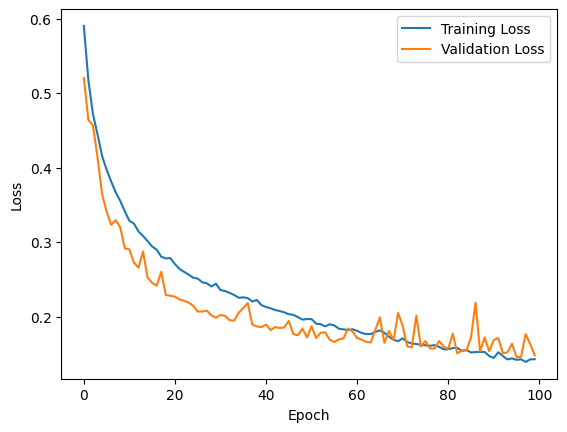
\includegraphics[width=0.75\textwidth]{loss_graph.png}
    \caption{Training-Validation Loss Graph}
    \label{fig:my_pic}
\end{figure}


\subsection{(10 Puan)} \textbf{SEED=öğrenci numaranız set ettikten sonra altıncı haftada ödev olarak verdiğim gibi earlystopping'deki en iyi modeli kullanarak, Prensesi İyileştir test setinden accuracy, F1, precision ve recall değerlerini hesaplayan kodu yazın ve sonucu da aşağı yapıştırın. \%80'den fazla başarı bekliyorum test setinden. Daha düşükse başarı oranınız, nerede hata yaptığınızı bulmaya çalışın. \%90'dan fazla başarı almak mümkün (ben denedim).}

\begin{python}
from sklearn.metrics import accuracy_score, f1_score, precision_score, recall_score

best_model = Net()
best_model = best_model.to(device)
checkpoint = torch.load('/content/checkpoint.pt')
best_model.load_state_dict(checkpoint)

predictions = []
ground_truths = []

with torch.no_grad():
  for inputs,label in testloader:

      inputs = inputs.to(device)
      label = label.to(device)

      output = best_model(inputs)

      for i in output:
        if(i < 0.5):
          predictions.append(0)
        else:
          predictions.append(1)
      
      for i in label:
        ground_truths.append(int(i))
      
f1_score = f1_score(ground_truths,predictions)
accuracy = accuracy_score(ground_truths,predictions)
precision = precision_score(ground_truths,predictions)
recall = recall_score(ground_truths,predictions)

print("F1-Score: {:.4f}\nAccuracy: {:.4f}\nPrecision: {:.4f}\nRecall: {:.4f}".format(f1_score,accuracy,precision,recall))
\end{python}

F1-Score: 0.9286
Accuracy: 0.9275
Precision: 0.9192
Recall: 0.9381

\subsection{(5 Puan)} \textbf{Tüm kodların CPU'da çalışması ne kadar sürüyor hesaplayın. Sonra to device yöntemini kullanarak modeli ve verileri GPU'ya atıp kodu bir de böyle çalıştırın ve ne kadar sürdüğünü hesaplayın. Süreleri aşağıdaki tabloya koyun. GPU için Google Colab ya da Kaggle'ı kullanabilirsiniz, iki ortam da her hafta saatlerce GPU hakkı veriyor.}

\begin{table}[ht!]
    \centering
    \caption{CPU-GPU Execution Times}
    \begin{tabular}{c|c}
        Ortam & Süre (saniye) \\\hline
        CPU & 55.0619 \\
        GPU & 49.0930\\
    \end{tabular}
    \label{tab:my_table}
\end{table}

\subsection{(3 Puan)} \textbf{Modelin eğitim setine overfit etmesi için elinizden geldiği kadar kodu gereken şekilde değiştirin, validasyon loss'unun açıkça yükselmeye başladığı, training ve validation loss'ları içeren figürü aşağı koyun ve overfit için yaptığınız değişiklikleri aşağı yazın. Overfit, tam bir çanak gibi olmalı ve yükselmeli. Ona göre parametrelerle oynayın.}

Modelin overfit etmesi için learning rate değerini 0.001'den 0.03'e yükselttim. Böylece model optimum noktayı kaçıracaktır. Aynı zamanda overfit miktarını arttırması için epoch sayısını da yükselttim. Overfit olayının daha iyi gözlemlenebilmesi için early stopping olmayan kodda çalıştırdım.
\\
\\
\\
\\
\\
\\
\\
\\
% Figür aşağı

\begin{figure}[ht!]
    \centering
    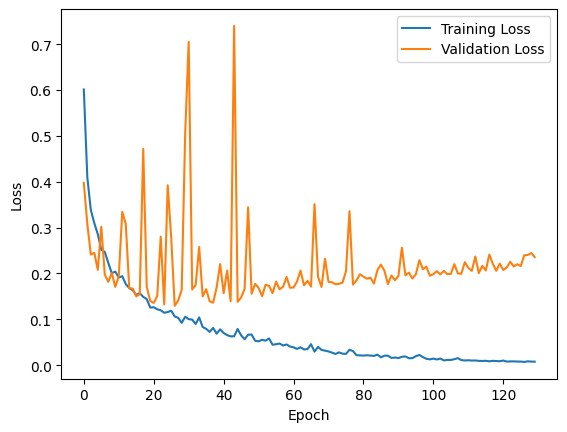
\includegraphics[width=0.75\textwidth]{overfitting.png}
    \caption{Overfitting Graph}
    \label{fig:my_pic}
\end{figure}


\subsection{(2 Puan)} \textbf{Beşinci soruya ait tüm kodların ve cevapların olduğu jupyter notebook'un Github linkini aşağıdaki url'e koyun.}

\url{https://github.com/onuroner/YapaySinirAglari_MLP}

\section{(Toplam 10 Puan)} \textbf{Bir önceki sorudaki Prensesi İyileştir problemindeki yapay sinir ağınıza seçtiğiniz herhangi iki farklı regülarizasyon yöntemi ekleyin ve aşağıdaki soruları cevaplayın.} 

\subsection{(2 puan)} \textbf{Kodlarda regülarizasyon eklediğiniz kısımları aşağı koyun:} 

\begin{python}
class Net(nn.Module):
    def __init__(self):
        super(Net, self).__init__()
        self.fc1 = nn.Linear( 13, 100 ) 
        self.fc2 = nn.Linear( 100, 50 )
        self.fc3 = nn.Linear( 50, 1 ) 

        self.relu = nn.ReLU()
        self.sigmoid = nn.Sigmoid()

        self.dropout1 = nn.Dropout(p=0.4) #REGULARIZATION
        self.dropout2 = nn.Dropout(p=0.2) #REGULARIZATION

    def forward(self, x):
        x = self.fc1(x)
        x = self.relu(x)
        x = self.dropout1(x) #REGULARIZATION

        x = self.fc2(x)
        x = self.relu(x)
        x = self.dropout2(x) #REGULARIZATION

        x = self.fc3(x)
        x = self.sigmoid(x)
        return x

model = Net()

LEARNING_RATE=0.001
EPOCHS=100

criterion = nn.BCELoss()
optimizer = torch.optim.SGD(model.parameters(), lr=LEARNING_RATE, weight_decay=0.001) #REGULARIZATION

train_losses = []
val_losses = []

model = model.to(device)
for epoch in range(EPOCHS):

  train_loss = 0.0
  val_loss = 0.0
  train_count = 0.0
  val_count = 0.0
  
  model.train()
  for inputs, labels in trainloader:
      #training loop
      inputs = inputs.to(device)
      labels = labels.to(device)

      optimizer.zero_grad()

      outputs = model(inputs)
      labels = labels.unsqueeze(1)
      loss = criterion(outputs, labels)
      loss.backward()
      optimizer.step()

      train_count += 1.0
      train_loss += loss.item()
    

  model.eval()
  with torch.no_grad():
    for inputs, targets in valloader:
      #validation loop
      inputs = inputs.to(device)
      targets = targets.to(device)
      
      outputs = model(inputs)
      targets = targets.unsqueeze(1)
      loss = criterion(outputs, targets)

      val_count += 1.0
      val_loss += loss.item()

    # epoch kayiplarini ekrana yazdir
  train_loss /= train_count
  val_loss /= val_count
  print(f"Epoch {epoch+1} train loss: {train_loss}, validation loss: {val_loss}")

  train_losses.append(train_loss)
  val_losses.append(val_loss)

torch.save(model.state_dict(), "checkpoint.pt")
plt.plot(train_losses, label='Training Loss')
plt.plot(val_losses, label='Validation Loss')
plt.xlabel('Epoch')
plt.ylabel('Loss')
plt.legend()
plt.show()
        

print('Finished Training')
\end{python}

\subsection{(2 puan)} \textbf{Test setinden yeni accuracy, F1, precision ve recall değerlerini hesaplayıp aşağı koyun:}

F1-Score: 0.8655
Accuracy: 0.8627
Precision: 0.8525
Recall: 0.8789

\subsection{(5 puan)} \textbf{Regülarizasyon yöntemi seçimlerinizin sebeplerini ve sonuçlara etkisini yorumlayın:}

Dropout kullanarak hidden layerlar arasında bazı nöronların eğitime katılmasını engelleyerek, weight decay kullanarak ağırlıkları küçülterek regularizasyon sağlamış oldum. Model loss grafiğine baktığımızda eğitimin daha yavaş ve stabil ilerlediği görülmektedir. Dalgalanmaların azaldığı, daha stabil bir eğitim sürecinin olduğunu göstermektedir.

\subsection{(1 puan)} \textbf{Sonucun github linkini  aşağıya koyun:}

\url{https://github.com/onuroner/YapaySinirAglari_Regularizaton}

\end{document}